\scanpage{11}
$T$ torseur \unsure{:|à} droite sous \unsure{grpe|grp} $\unsure{\mathbb{Z}|Z}$

\[
\deleted{\unsure{\operatorname{Aut}_{\substack{G\text{-ens}\\G\text{-}\unsure{\mathrm{var}|\mathrm{op}}}}(\unsure{D|T})
 \longrightarrow\operatorname{Aut}(G)}}
\]

\diagram{\begin{tikzcd}[ampersand replacement=\&,column sep=small]
1\arrow[r] \& \mathbb{Z}\arrow[r,"i"] \& \operatorname{Aut}(\mathbb{Z},T)\arrow[r,"p"]
 \& \operatorname{Aut}(\mathbb{Z})\arrow[r,dash]\arrow[l,dashed,bend left=28,"q_t"'] \& 1
\end{tikzcd}}

% A detached dark trace stands above un; its attribution to writing is uncertain.
$\forall t\in T$, on a
\tikz[baseline=(unword.base)]{
\node[inner sep=0pt] (unword) {un};
\node[inner sep=0pt] at ([xshift=.35em,yshift=1.45em]unword.base)
 {\unsure{\rule{.12em}{.055em}}};}
splitting $q_t$, défini par
\[
\left\{\begin{aligned}q_t(\gamma)(t)&=t\\p(q_t(\gamma))&=\gamma\end{aligned}\right.
\]

Quelle est la relation entre $q_t$ et $q_{t'}$ ?

On \unsure{avait|aurait} $t'=t.g$, et on trouve
\[
q_{t'}=\operatorname{int}(i(g))\circ q_t
 \;:\; \gamma\longrightarrow i(g)\,q_t(\gamma)\,i(g)^{-1}
\]

[ Pour le vérifier, il suffit de voir que
\[
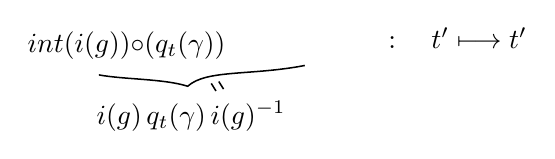
\begin{tikzpicture}[x=.012cm,y=-.012cm,baseline=0]
\node[anchor=base west,inner sep=0pt] at (0,0)
 {$\operatorname{int}(i(g))\unsure{\circ}(q_t(\gamma))$};
\node[anchor=base west,inner sep=0pt] at (382,-4)
 {$:\quad t'\longmapsto t'$};
% The brace covers only the middle of the expression, as drawn.
\draw[line width=.55pt] (76,24)
 .. controls (104,29) and (145,28) .. (170,36)
 .. controls (190,18) and (237,25) .. (294,14);
% Two separate slanted strokes form the equality below and right of the cusp.
\draw[line width=.55pt] (195,33)--(200,41);
\draw[line width=.55pt] (203,31)--(208,39);
\node[anchor=base west,inner sep=0pt] at (73,76)
 {$i(g)\,q_t(\gamma)\,i(g)^{-1}$};
\end{tikzpicture}
\]
or \quad $t'=tg$
\[
\begin{aligned}
&\deleted{q_t(\unsure{\gamma})(t')=q_t(\gamma)(t)\,\gamma(g)=t.\gamma(g)}\\
&\deleted{\operatorname{int}(i(g))\,q_t(\gamma)\,(t')=}\\
&i(g)^{-1}(t')=t\qquad q_t(\gamma)\,i(g)^{-1}(t')=q_{\unsure{b|t}}(\gamma)\,t=t\\
&i(g)\,q_t(\gamma)\,i(g)^{-1}(t')=tg=t'\qquad\text{ok}\qquad ]
\end{aligned}
\]

\reversemarginpar
\margin{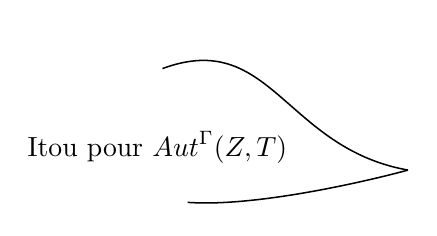
\begin{tikzpicture}[x=.01cm,y=-.01cm,baseline=0]
\node[anchor=base west,inner sep=0pt] at (0,0)
 {Itou pour $\operatorname{Aut}^{\Gamma}(\mathbb{Z},T)$};
\draw[line width=.55pt] (172,-112)
 .. controls (310,-163) and (327,-11) .. (484,17);
\draw[line width=.55pt] (204,58)
 .. controls (286,64) and (421,34) .. (484,17);
\end{tikzpicture}}
\normalmarginpar

\[
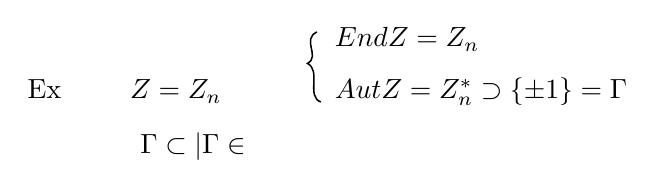
\begin{tikzpicture}[x=1cm,y=1cm,baseline=0]
\node[anchor=base west,inner sep=0pt] at (0,0) {\uline{Ex}};
\node[anchor=base west,inner sep=0pt] at (1.3,0) {$\mathbb{Z}=\mathbb{Z}_n$};
\node[anchor=base west,inner sep=0pt] at (3.9,.66) {$\operatorname{End}\mathbb{Z}=\mathbb{Z}_n$};
\node[anchor=base west,inner sep=0pt] at (3.9,0)
 {$\operatorname{Aut}\mathbb{Z}=\mathbb{Z}_n^{*}\supset\{\pm1\}=\Gamma$};
\draw[line width=.55pt] (3.68,.85)
 .. controls (3.48,.75) and (3.73,.54) .. (3.56,.45)
 .. controls (3.74,.36) and (3.54,.03) .. (3.73,-.04);
\node[anchor=base west,inner sep=0pt] at (1.43,-.70)
 {$\deleted{\unsure{\Gamma\subset|\Gamma\in}}$};
\end{tikzpicture}
\]
\margin{\begin{tabular}{@{}l@{}}
(\uline{NB} \unsure{si} $n=2$, $+1=-1$\\
\quad dans $\mathbb{Z}_n^{*}$\ldots)
\end{tabular}}

\[
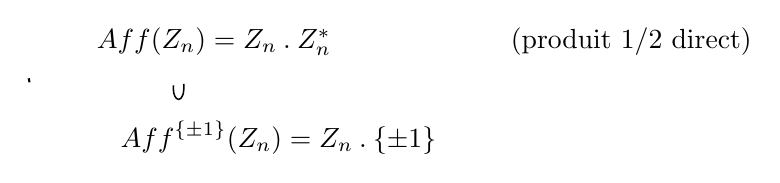
\begin{tikzpicture}[x=.01cm,y=-.01cm,baseline=0]
\node[anchor=base west,inner sep=0pt] at (0,0)
 {$\operatorname{Aff}(\mathbb{Z}_n)=\mathbb{Z}_n\mathbin{.}\mathbb{Z}_n^{*}$};
\node[anchor=base west,inner sep=0pt] at (526,0)
 {(produit $1/2$ direct)};
% Open upward stroke between the formulas, without an assigned set-operation meaning.
\draw[line width=.55pt] (98,47)
 .. controls (96,70) and (113,72) .. (111,45);
% Detached short dark stroke to the left of the interline relation.
\draw[line width=.75pt] (-86,38)--(-85,43);
\node[anchor=base west,inner sep=0pt] at (30,126)
 {$\operatorname{Aff}^{\{\pm1\}}(\mathbb{Z}_n)=\mathbb{Z}_n\mathbin{.}\{\pm1\}$};
\end{tikzpicture}
\]
\margin{\begin{tabular}{@{}l@{}}
groupe \unsure{diédral|diédhral}\\
d'indice $n$, $\mathbb{D}_n$\\
(on suppose $n\ne2$\ldots)
\end{tabular}}

Soit $T$ torseur sous $Z$ groupe cyclique d'ordre $n\geq3$ muni d'une famille $\{u,u^{-1}\}$ de 2 gén.
\tikz[baseline=(old.base)]{
\node[anchor=base west,inner sep=0pt] (old) at (0,0)
 {\deleted{\unsure{d'ordre $n$}.}};
\node[anchor=south west,inner sep=0pt] at ([yshift=.14em]old.north west)
 {\inserted{inverses l'un de l'}};}
autre.
\diagram{\begin{tikzcd}[ampersand replacement=\&,column sep=small]
1\arrow[r] \& Z\arrow[r,dash,"i"] \& \operatorname{Aut}^{\pm1}(T,Z)\arrow[r,dash,"p"]
 \& \{\pm1\}\arrow[r,dash]\arrow[l,bend left=25,"q"] \& 1
\end{tikzcd}}
% archive sheet number: 10
